\chapter{The Analog Subsystem}

Analog? Yes, there is analog. Although the Layout Control System is a digital system with locomotives controlled via DCC, there are cases where implementing a layout based on controlling all rolling stock via DCC would mean to equip all your analog running engines with DCC decoders. Besides that it represents quite a considerable cost and converting some older locomotives is a real project in itself. Also, there are model railroad clubs with literally hundreds of locomotives. These layouts are analog and you will find miles of cables to a central control station. Converting all of the existing infrastructure in one swoop represents a considerable cost.

This chapter presents an overview for a subsystem managing analog locomotives. We will only focus on analog running equipment. Devices such as signals, turnouts and other stationary equipment is managed with the LCS node, port, event system, i.e. digital. This chapter will introduce extensions required to manage an analog and also a potentially hybrid layout.

\section{Requirements}

The first major difference to a DCC based system is that for a given track section there can only be one locomotive or consist. In contrast to a digital signal with a permanent flow of the square wave signal, an analog system will use a pulse width modulated (PWM) approach. A wider pulse width will make the engines run faster, a smaller pulse width makes it run slower. The signal contains no information about the actual engine and just delivers power corresponding to speed desired to the track section.

To still run several engines, the layout needs to be divided into several sections or blocks. Just as we divided a layout into sections with separate DCC boosters, analog layouts will control sections with a separate power module. It is not necessary to have a power module for each section, but the more sections and power modules the more analog engines could run simultaneously. Built on top, an analog layout often has a concept of blocks to run trains automated managed by a block signal control system. The blocks are often divided further into subsections and there are track occupancy detectors to know where the loco is within the block.

Just like their DCC cousin, analog track sections need special consideration when an engine is moving from one block to the next. For DCC track sections, each having a booster receiving the same DCC signal from the base station, there is a short window of power disconnect to address any small booster timing differences. For the analog world, the current section and the following one need to be also in sync for the engine to cross from one block to the next. The PWM signals, which deliver the power to the locomotive, need to be synchronized in order to avoid that one block still delivers power and the next block not quite yet. A locomotive would not run smoothly in that case.

An analog track block would also need to know the actual engine characteristics of the engine in a block. Each engine has different power consumption characteristics, so the speed is a function of engine type and actual train load. This track control mechanism is very closely associated with an overall block signaling control system. In fact, an analog system almost every time has a block signaling system implemented to manage several engines. Note that in an analog the smarts must be in the block controller and not in the engine. In a DCC system, the smarts is in the engine. In A DCC system the booster are there to address the overall power needed, dividing a layout into several power sections. In an analog system, the sections are there to address the need to run many engine simultaneously. There can only be one engine in a track sections or block.

There is also the situation that a layout is in a transition from analog to digital. Wouldn't it be nice to manage both worlds in the same layout? A block could either host a DCC equipped locomotive or an analog locomotive, but never at the same time. Also, it needs to be ensured that the follow-on block where the engine is heading is of the right kind. This is brings up several more design questions, and we will talk about it in the following sections.

In any case, an analog system also needs a means of a cab handheld to control the engine. Following the LCS overall concept, the communication between the cab handheld and the layout nodes that ultimately control the engine, is digital. The concept of a locomotive session and a base station that manages all active sessions supports both DCC as well as analog engines. The base station managing locomotive sessions would need to be enhanced slightly to also support analog running equipment. Of course the cab handheld for an analog locomotive is much simpler. All that is needed is the direction and speed control.

\section{Overall concept}

Before diving into details, this section shows how support for an analog system could be implemented. There is the basis station managing all active locomotive sessions. The cab handheld will broadcast the speed / direction LCS message, which is received by the base station and translated to a DCC command packet sent out via the LCS bus. From an overall perspective, there is no difference in managing a locomotive session. There is still a handheld to set the speed and direction and there is a central place that is aware of all active sessions.

However, an analog engine has no concept being directly addressable. The typical solution is to divide the track into sections and control the sections where the locomotive currently is. The section is called a block and a block itself consist of one or more sub sections. The track subsections each have a sensor to detect that there is something drawing current from the track and the block controller has a way to know which locomotive is in which block. The following figure depicts an analog layout using the LCS components.

picture 

\begin{figure}[!ht]
    \centering
   % 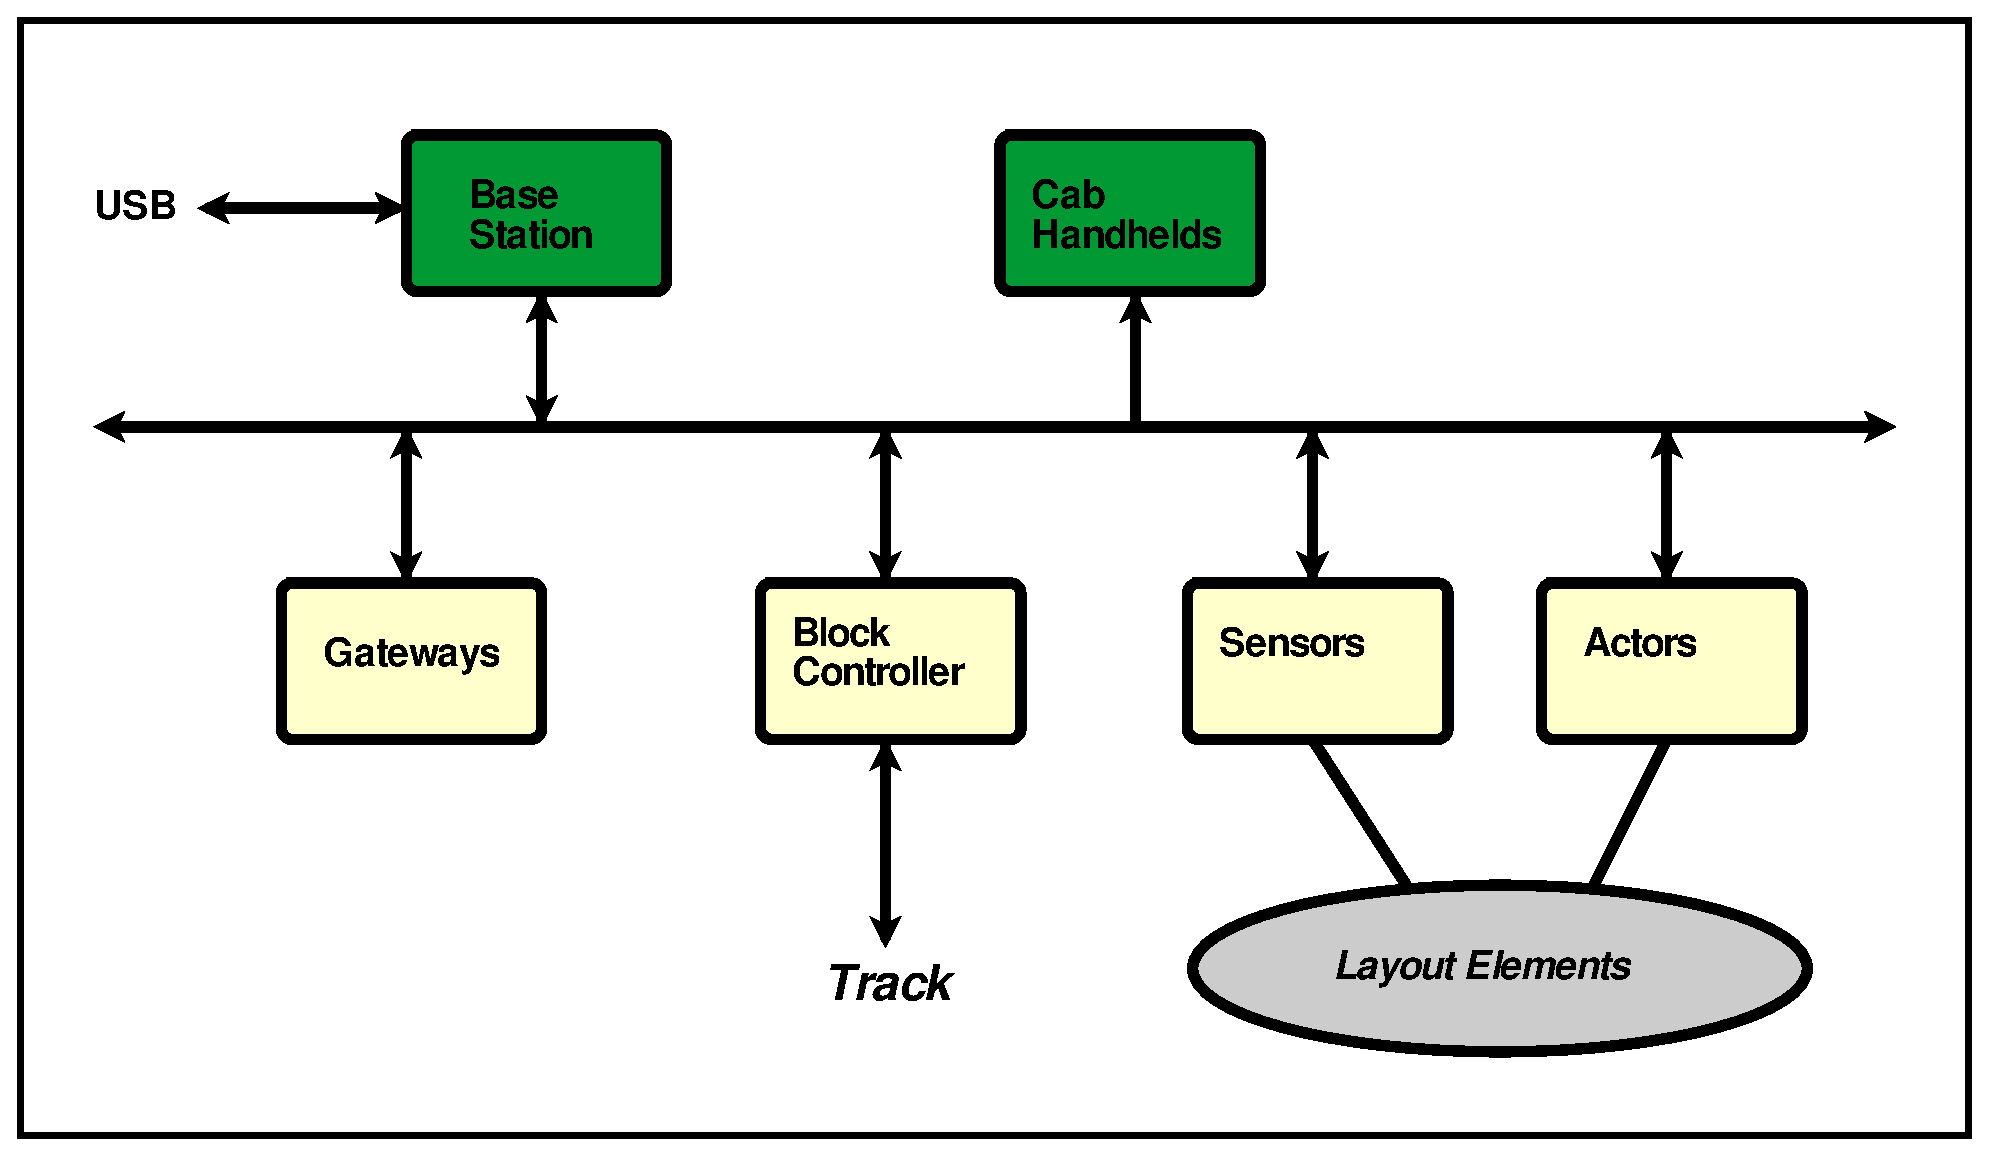
\includegraphics[page=1, width=\textwidth]{./figures/Schematic_LcsNodes-Layout-Overview.pdf}
   %![Schematic_LcsNodes-Analog-Block-Control.png](./Figures/Schematic_LcsNodes-Analog-Block-Control.png )
\end{figure}

The LCS base station that manages all active locomotives, will not work differently for a digital or analog locomotive. It will create a session and also emit DCC data packets for controlling among other thongs speed and direction. The DCC signal is broadcasted via the LCS bus. This way it will also reach all block controllers that manage a block. The block controller will then decode the DCC packet and if it concerns a locomotive that according to the block controller data is currently in the block will put the respective PWM signal on the track. This is different to a normal DCC booster. A DCC booster just amplifies the incoming DCC signal and puts it onto the track. A block controller will decode the DCC signal and put a corresponding PWM signal on the track.

\section{Locomotive session management}

For each active locomotive the base station first establishes a locomotive session. Across the layout, a locomotive is uniquely identified by its **cabId**. Once a session is established for the cabId, the base station accepts LCS commands for setting the speed and direction. This is common to both the DCC digital and analog control of a locomotive as far as the base station is concerned. The only difference is that for an analog engine, only speed and direction can be set. All other capabilities such as sound control and functions for turning on and off a headlight are not available.

\section{Analog Track Signal Generation}

The analog track signal does not contain any information transmitted via the signal. The signal is just a pulse width modulated electrical current. The wider the pulse the faster the engines will go. The direction is determined through the polarity of the track. Just like emitting a DCC signal waveform, the H-Bridge of the power modules can easily also emit a pulse width signal with the right polarity. Short circuit detection and power consumption measurement work independent of the kind of signal emitted.

\section{Analog Track Blocks and Track subsections}

Layouts with analog engines will almost certainly have a number of blocks that can be powered individually. There is a one to one relationship of a power module with a block. A block is further divided into a number of track subsections with occupancy detectors, so the locations where power is drawn within the block can be determined. The chapter on block controller and block signaling will pick up this topic in more detail.

Just like the DCC subsystem, care needs to be taken when a locomotive crosses from one block fed from a power module to the next block fed by another power module. The actual current put on the tracks needs to be in sync, such that there is not awkward jump or worse current flow between the blocks connected via the locomotive wheels when crossing. It needs a way of synchronizing the PWM signals. Classic analog block control system transmitted a separate signal for all block controllers. In our world, the DCC signal emitted to all block controller nodes throughout the LCS layout via the LCS bus is our synchronization method.

\section{A short Glimpse at Software Implementation}

The block controller is the heart of managing a block in an analog layout. It will be responsible for managing the track block with a number of subsections. Using the LCS event system, blocks communicate and broadcast data about the locomotive entering and leaving their block. Using defined node and port attributes, they also communicate about block occupancy. Turnout control and position feedback as well as track signal control are also be the part of the duties of a block controller.

A part of the block controller firmware will decode LCS messages to determine if there is a command that concerns a locomotive that according to the block controller data is currently managed by that block. Note that there is no way to really know that this is the locomotive until there is some mechanism of identifying a locomotive when entering a block. For example, the sending block where the locomotive is coming from sends an event that this locomotive has left the block. Consequently, the receiving block knows the locomotive ID and broadcasts the event of arrival.

Another part of the block controller firmware needs to manage the power module. Depending on the locomotive characteristics the speed and direction are set. Short circuiting and power consumption are measured just like it is done in a DCC subsystem. I addition the PWM signal phase needs to be the same in all blocks. This is accomplished by a common synchronization signal.

Finally, the firmware will track that a train truly left the block. This information is a combination of the follow-on block indicating that the train entered and a computed time interval where the train should have completely left the previous block has passed. If this is not the case, perhaps the train derailed or a part of it decoupled.

\section{Summary}

Analog systems have their purpose also in a digital world. The approach taken by the Layout Control Systems is to put the smarts of managing the running equipment of such a layout into a set of block controllers with the base station and cab handhelds transparently supporting DCC equipped and analog engines. Both worlds use the power module for managing the track current delivery and consumption measurement. While for DCC the power module generates an amplified copy of the DCC signal, it will generate a PWM signal for an analog engine.

The block controller takes on part of the duties of a DCC locomotive decoder in a digital layout. The DCC signal broadcasted to all nodes in the layout is simply decoded and matched with the locomotive information of the respective block controller. All block controllers constantly broadcast via the LCS event mechanism their current state.

Not discussed yet, there needs to be a central configuration system that keeps all the data about all blocks and their relation to each other. There also needs to be a dictionary of all locomotives and their characteristics. On top configuration software and also panels to set track routines and so on. The requirements will be discussed in the block signaling chapter.
